\documentclass[11pt]{article}
\usepackage{graphicx}
\oddsidemargin 1mm

\textwidth 6.3in 
\topmargin -5mm
\headheight 5mm 
\headsep 8mm
\textheight 8.9in

\renewcommand{\baselinestretch}{1.0}
\parindent 0pt
\parskip  4pt

%%=========================================================
\begin{document}
\noindent
\thispagestyle{empty}
\sloppy

\rule{1mm}{0mm}

\vspace{-17mm}
{\LARGE \bf Prosody Principal Components Analysis (PPCA) }
\medskip


{\LARGE \bf Version 4.1}
\vspace{7mm}


{\bf Nigel Ward, University of Texas at El Paso and Kyoto University}

{\bf \today }

%\bigskip
%\noindent
%Abstract: Applying Principal Component Analysis to prosodic features
%has been useful for several tasks.  This report describes the
%Matlab-based workflow and code.


\begin{tabular}{p{7cm}l}
& 1 Background  \\
& 2 Overview \\
& 3 File Formats \\
& 4 Visualization and Interpretation \\
& 5 Internals\\ 
& 6 Validation \\
& 7 History \\
& 8 Future Work \\
& 9 Local Notes
\end{tabular}


%%=========================================================
\section{Background} 

This document describes a toolkit for the doing things with prosody in
dialog.  It has three unique features: a novel set of prosodic
features \cite{mid-level-features}, support for Principal Components
Analysis (PCA), anad a large number of functions to support automated
and human-in-the-loop analyses.

We have found Principal Components Analysis, applied to a large set of
prosodic features spanning various temporal windows, to be useful for
various purposes.  It gives dimensions which correspond to
interpretable patterns of behavior \cite{prosodic-elements}.  The
values of these dimensions usefully characterize the instantaneous
state of the dialog \cite{dialog-dimensions}.  Applications so far
include language modeling, information retrieval, filtering, gaze
prediction, distributional analysis, predicting actions from prosody,
and examining non-native dialog patterns
\cite{pca-lm,prosody-ir,sigdial-codec,ward-vcip,dimensions-uh-huh}.

This document is written for three audiences: people wanting to learn
how this works, people wanting to get the code working for themselves,
and people wanting to modify or extend the code.


%==========================================================
\section{Overview}

There are two main use cases.  Figure \ref{diagram} overviews how they
relate.

\begin{figure*}[tp]
 \centerline{ 
 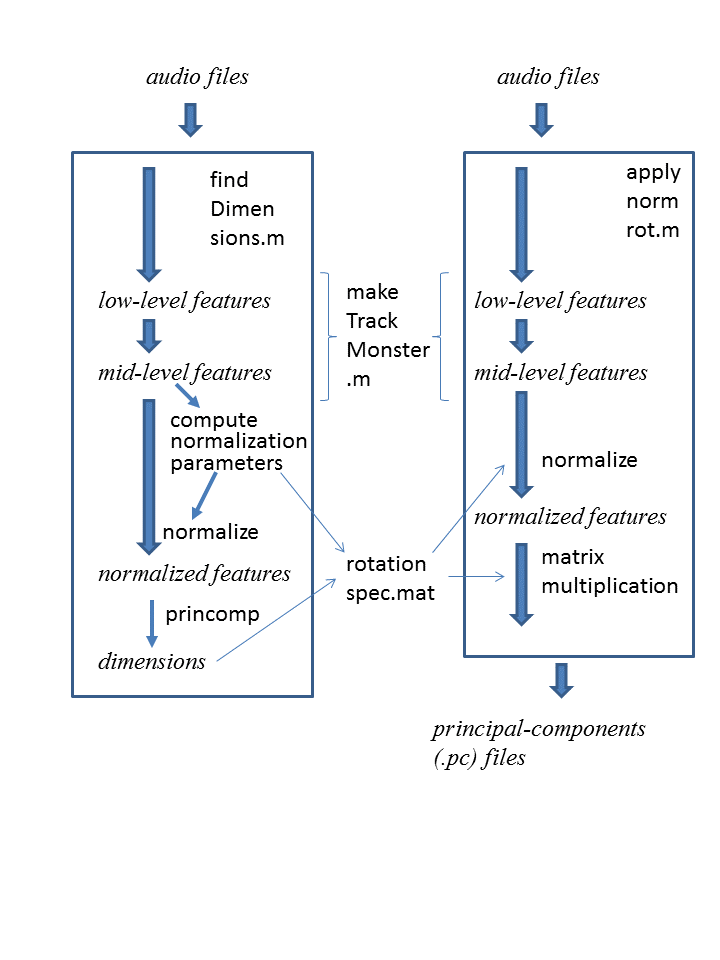
\includegraphics[width=11.4cm, trim = 1.cm 4.9cm 0cm 4.05cm, clip=true]{workflow-overview}
}
\caption{Workflow Overview}
\label{diagram}
\end{figure*}


%-------------------------------------------------------
\subsection{Apply Rotation}    \label{applynormrot}
 
This computes, for each moment of a dialog, the values of the
principal components at that moment.  For most purposes this will be
done using some standard, pre-computed principal components, together
with some standard normalization parameters.  (The results may make
more sense if the file to be processed is from the same set as the
audio used to generate the normalization parameters (Section
\ref{computerotation}), thus avoiding potential problems due to
different domains, speaking styles, or languages.  Recording
conditions may also be an issue, although the features are designed to
be somewhat robust to these.)

Thus the Matlab function {\tt applynormrot.m} creates a {\tt .pc} file
for each track of one or more audio files.  The steps are:
\begin{itemize}   \setlength{\itemsep}{0pt}\setlength{\parskip}{0pt}
\item read in an audio file (or set of files; this is the training corpus)
\item compute the raw  features
\item normalize them, using some precomputed parameters (means and
  standard deviations)
\item  rotate them, using a precomputed rotation
\item  write the results to {\tt .pc} files.
\end{itemize}

The resulting dimensional representation can then be as input to
machine-learning algorithms for various tasks, or can be interpreted.

%$\clubsuit$ every invocation of findDimensions.m or applynormrot.m,
%should be documented in and automatically-created logfile, including
%timing information, written to the same directory the .pc files are
%in, as additional provenance beyond the on-line header.

%------------------------------------------------------------------
\subsection{Compute Rotation} \label{computerotation}

In order to do the above, there of course needs to be a
normalization-and-rotation available to work with.  {\tt
  findDimensions.m} creates this.  The steps are:
\begin{itemize}   \setlength{\itemsep}{0pt}\setlength{\parskip}{0pt}
\item read in an audio file 
\item compute the raw  features
\item compute normalization params, then use them to normalize the features
\item compute the rotation, that is, do PCA to discover the dimensions
\item save the rotation coeffs and the norm params for later use (Section \ref{applynormrot})
\end{itemize}

%------------------------------------------------------------------
\subsection{Overview of the Arguments}   \label{arguments}

In general, there are five things needed to completely specify either
of these processes.  Three of these are arguments:

\begin{description}  \setlength{\itemsep}{0pt}\setlength{\parskip}{0pt}
\item[tracklist] specifies which tracks to process, each being a
  track from an audio file (Section \ref{tracklist-files})
\item[featurespec file]  specifies the set of features to use (Section \ref{featurespec-files})
\item[output dir] specifies where to write the resulting {\tt .pc}
  files (one per track), and extremes files (one per dimension)
\end{description}

The other two things are locations which set implicitly. 

\begin{description}  \setlength{\itemsep}{0pt}\setlength{\parskip}{0pt}
\item[pitch cache] subdirectory where to store (or find) the {\tt
  fxrapt}-output f0 values, as {\tt .mat} files.  This subdirectory is
  created in the same directory where the audio files are located, as
  specfied in the featurespec file.
\item[parameter dir] directory where to store (or find) the params and
  coeffs (notably in the file {\tt rotationspec.mat}, and the various
  human-readable files, notably the logfile, correlation coefficients,
  and factor loadings.  This directory is implicitly set to be the
  location where the matlab process is run.
\end{description}

Given the implicit storing of the params and coeffs, it's probably
best to create a new directory for each project.  If all relevant
Matlab work is done in this directory, then all the parameter files
will be written here and then found again without difficulty.


%%=========================================================
\section{File Formats}       

%--------------------------------
\subsection{Data Files}

First there are the data files, each representing an audio track or
file, at various stages of processing.

\begin{description}   \setlength{\itemsep}{0pt}\setlength{\parskip}{0pt}

\item [---.au, .wav] The input.  A stereo audio file.  Since {\tt
  .wav} files sometimes cause trouble for {\tt fxrapt}, it's safer to
  convert everything first to {\tt .au} format.  Traditionally these
  have been in Sun format, specifically 16 bit, linear PCM, 8K
  sampling.

\item[---f0.mat] a file specifying for an audio track the pitch every
  10 milliseconds.  These files are created because fxrapt is slow, so
  it's worth saving the results to avoid needing to later recompute
  them.

\item[---.pc] The output: a principal components file.  There is a
  one-line header describing the provenance.  Each subsequent line
  describes the prosody at one timepoint.  These are 10ms apart.  Each
  line contains a whitespace-separated list of, first the timepoint,
  then the values for all the principal components (PCs).  PCs appear
  in order of the variance explained.  These files are large and
  writing them takes a long time, so this function is currently
  commented out.
\end{description}


%%=========================================================
\subsection{Tracklist Files}       \label{tracklist-files}

This specifies the audio tracks to process.  The first line is the
directory in which the audio files are located.  Subsequent lines
specify the track and the file.  For example the line

\begin{quote}
\verb+l sw02079.au+
\end{quote}

means to process the left track of the specified Switchboard audio
file.  Tracklist files have the extension {\tt .tl}. 


%%=========================================================
\subsection{Feature Specification Files}     \label{featurespec-files}

To encode contextual information we need to use features computed at
various temporal offsets, relative to the point of interest.  A
``featureset specification'' ({\tt .fss}) file specifies which
features to use.  These are sometimes called ``crunch'' files since
originally they described how to crunch together data from individual
feature files into a single composite file suitable for machine
learning or dimensionality reduction.

Various {\tt .fss} files exist, including {\tt fulltest/al.fss}, an
``assumption light'' new set of mid-level features, including about
168 features, and {\tt comparisons/april.fss}, which has more features
for the primary-track talker than for the other talker. 

% need to ensure that the .fss files get included in a future 
% distributions

In a {\tt .fss} file each line specifies a feature, a window size, and
an offset, for example

\begin{quote}{\tt 
    vo   -100   -200 self  \\
    cr   -200    400 inte
}\end{quote}

where the first line means the speaker's average volume over a 100ms
window that starts 200ms before the point of interest, and the second
line the interlocutor's average creakiness over a 200ms window that
starts 400ms after the point of interest.  

In these files currently the following codes are recognized:

New two-letter codes: 

\begin{tabular}{ll}
  vo  & intensity/volume \\
  sr  & speaking rate proxy \\
  cr  & creakiness \\
  fp  & flat pitch: degree of flatness \\
  np  & narrow pitch range: degree of narrowness \\
  tp  & typical pitch range \\
  wp  & wide pitch range  \\
  hp  & high pitch (obsolete) \\ 
  lp  & low pitch (obsolete) \\
  th  & true high pitch: degree of highness (obsolete) \\ 
  tl  & true low pitch: degree of lowness (obsolete) \\
\end{tabular}

Reserved two-letter codes: 

\begin{tabular}{ll}  
  sf      & speaking fraction \\
  vf      & voicing fraction \\
  p0...p5 & pitch bands, as a potential replacement for lp and hp  \\
  sl      & slowness, to replace sr \\
  fa      & fastness, ditto\\
\end{tabular}

Adding a new prosodic feature requires changing three things.  First
you create an entry for your new feature in the featurespec file,
choosing any convenient two-letter code and an appropriate window size
and offset.  Second, you write a new matlab function to compute that
feature.  This might compute it from the audio, or from other
features, or it might read values from a file that was written by an
external program.  Third, you add a new case to the big switch in {\tt
  makeTrackMonster} to associate your new feature-computing function
with the two-letter code.

Every feature-computing function is responsible for returning a vector
of values for windows centered every 10 milliseconds throughout the
audio file.  The first one is centered at 10 ms.  This is true for
both the frame-level features (energy and pitch) and for the derived
(mid-level) features, which span longer windows.  While the raw pitch
features can include NaNs, this is not allowed for the mid-level
features.

Thus all feature-computing functions must return values everywhere,
even at the start and end of the audio file.   Mid-level features
have windows longer than 20ms, so windows centered close to the start
or end of a file will stretch out beyond the point of no data, and
thus they will lack enough information to return a well-considered
value.  In such cases the function should return zero or some other
non-obtrusive value in the typical range (rather than some extreme
value like -9999 as a flag, since that would mess up the
normalization).  While the code could be more careful this, it's not a
problem for now, since all audio files we work with are long enough
that the vast majority of data values will be valid.


%%=========================================================
\subsection{Normalization and Rotation Parameter File}

{\tt rotationspec.mat}  contains the information pertaining to a
rotation.  This enables the application of an pre-determined rotation 
to new files.  It contains 

\begin{itemize}  \setlength{\itemsep}{0pt}\setlength{\parskip}{0pt}
\item the normalization parameters, namely for each feature its mean
  and its standard deviation

\item the PCA coefficients
\end{itemize}

A related file is {\tt loadings.txt}, which is a human-readable
version of the PCA coefficients.


%==================================================================
\section{Support for Examining and Interpreting the Results}

Examination of intermediate and final results is important, both to
check that everything is working properly, and to interpret the
results of the process.

%--------------------------------------------
\subsection{Examining the Features}

To see the values of various low-level and mid-level features as they
vary over an audio file, uncomment the various {\tt plot} commands in
{\tt makeTrackMonster.m}.  One can then listen to the audio file,
using any available player, to see whether the feature values are
indeed high and low where they should be.

%--------------------------------------------
\subsection{Examining the Correlations}

As an indirect check on correctness of the feature computation and
collating, one can examine the correlations among the features.  Every
call to {\tt findDimensions.m} creates two correlation files: {\tt
  pre-norm-corr.txt} and {\tt post-norm-corr.txt}, each showing the
most highly correlated and most anticorrelated features for each othe
feature.  These are output by {\tt output\_correlations.m}.

%--------------------------------------------
\subsection{Examining Statistics about the Dimensions}

To see the variance and cumulative variance explained by the PCA-found
dimensions, load the {\tt rotationspec.mat} file and process it with:

\begin{quote}
\begin{verbatim}
load rotationspec
latent ./ sum(latent) 
cumsum(latent) ./ sum(latent) 
pareto(latent ./ sum(latent))   # produces a cool graph
\end{verbatim}
\end{quote}

More interestingly, for each dimension, we'll want to examine
individual variation and (somewhat later) group variation.  The
between-groups comparison will compare all learner data with all
native data, in terms of the two summary statistics, to find out which
dimensions they differ on.

The summary statistics are:
\begin{itemize}   \setlength{\itemsep}{0pt}\setlength{\parskip}{0pt}
\item average value (to detect bias to one side of the dimensions)   
\item standard deviation (to detect failure to use a dimension much)
\item skewness
\item kurtosis
\end{itemize}

This is done by {\tt write\_summary\_stats.m}, whose input is the
rotated matrix.  For each column of the matrix (each feature), we
compute these things.  This is called by {\tt applynormrot.m}.  There
is also fragments of a workflow described in {\tt histo/README.txt}:
in short, this uses {\tt distDist.m}, {\tt bhatd.m}, and {\tt
  binProbs.m} to generate histograms for each dimension, including
superimposed histograms for the two populations, and to compute the
Bhattacharyya distance.


%--------------------------------------------
\subsection{Interpreting the Dimensions}

To understand the dimensions, there are three methods to apply.

%---------------------------------
\subsubsection{Examine the Factor Loadings}

{\tt findDimensions.m} includes a call to {\tt writeloadings.m}, which
writes a large, human-readable file called {\tt
  loadings.txt}, the lines of which give the loadings of each feature on each
dimension, for example:

\begin{verbatim}
dimension1  0.12 sel-vo-50+0
dimension1 -1.08 int-ph-400-200
dimension1  0.01 sel-pr+50+100
...
dimension2  0.67 sel-sr+0+100  
...
\end{verbatim}

These files can then be examined to understand the nature of each
dimension.  It's particularly useful to first look at the volume features (with
{\tt grep}) for the ``self'' speaker, to find out when they're
talking.  A useful next step is to look at the ``interloc'' volume
features.  Next it's useful to use the Unix {\tt sort} and {\tt grep}
commands to find, for example, the features with the highest loadings
and those with the strongest (highest absolute) loadings.  

There is also code to visualize the loadings of one dimension in {\tt
  patvis.m};  the {\tt diagramDimensions.m} function creates
visualizations for all dimensions.


%---------------------------------
\subsubsection{Listen to Extreme Examples}

To understand a dimension, it helps to listen to locations in data
where each dimension has extreme (the highest and lowest) values.  To
support this, by examining the files {\tt dim00.txt} etc.\ in the {\tt
  extremes} subdirectory of outdir.  This is written by {\tt
  findExtremes.m} (called by {\tt applynormrot.m}).  This finds the
extreme points in each file, but winnows out points too close to each
other, to provide some diversity.

Once we have these timepoints, it's time to listen.  There are lots of
tools that can do this, but we want one that can easily let you jump
to 5 seconds before this point, then play this region.  Invokability
from the command line is a big plus.  Using second notation (not
minutes and seconds) is also nice.  Dede does these things, but only
seems to run on 32-bit linux machines with Centos/Redhat 5. One
version is in {\tt /home/research/isg/speech/workingDede/dede}.  If
dede crashes, copy {\tt
  /home/research/isg/speech/workingDede/piau-au-file.PCM } to {\tt
  /tmp} and restart it.

In future, it might be nice to automatically feed timepoints to {\tt
  dede}, to direct it to the right places without requiring the user
to view and re-specifiy timepoints.


%---------------------------------
\subsubsection{Consider Co-occurring words} 

The last source of insight for interpreting the dimensions is to see
find which words co-occur with values high/low on each dimension.  Of
course this is only possible if we have transcribed data,
e.g.~Switchboard.  A
workflow for this needs to be revived.


%%=========================================================
\section{Internals}

%--------------------------------------------
\subsection{Frame-Level Feature Computation}

The frame-level (low-level) features are computed: pitch and energy.

The pitch is done with {\tt lookupOrComputePitch.m}, which is a
wrapper for Mike Brookes's Voicebox function {\tt fxrapt.m}; this
gives values in hertz, or NaNs if there is no detectable pitch.

The low-level energy computation is done using {\tt
  computeLogEnergy.m}.

Other frame-level features may later be added.  For example this might
include features  generated by {\tt Praat} (notably NHR).  

If keystrokes are specified in the {\tt .fss} file, {\tt
  featurizeKeystrokes.m} is called to load that information; similarly
{\tt featurizeGaze.m} is called if gaze features are specified.

%--------------------------------------------
\subsection{Track-Based Normalizations}

Pitch is converted from hertz to percentiles, to normalize for
individual differences in pitch height and in pitch range.

Energy is rescaled to normalize for individual differences and
recording-condition differences in average speaking volume and in
average noise level.  To do this it finds the typical-silence and
typical-speech values of energy, using {\tt findClusterMeans.m} and
then normalizes the energy with respect to these values.  This is
done, not over the frame-level features, since those are probably too
short, but as part of the subsequent energy-over-larger-window
computations.

(This is not the simplest way to normalize, but it seems suitable.
The average volume across tracks will vary with the amount of speaking
the person in that track is doing.  Thus we want to ensure that each
person, when he is speaking, is reported has having the same volume on
average.  (This is of course not true, since some people have quieter
voices than others, but we can't really detect that.  Also that
probably doesn't matter, since we're only interested, for most
purposes, in whether a speaker is being quiet or loud relative to his
typical speaking volume.)  There may are also be slow variations in
gain, if the talker varies the handset-to-mouth distance, but these we
also don't deal with.


%--------------------------------------------
\subsection{Mid-Level Feature Computation}   \label{other-features}

The mid-level features are as listed in Section
\ref{featurespec-files}.  Each summarizes something about the values
of the frame-level features across some window.  The motivations for
these specific choices of feature are in \cite{mid-level-features}.

Each value is associated with the time at the center of the window.
Windows are shifted (stepped) every 10ms, because it's unlikely that
prosodic features change faster than that.  Windows are always at
least 50ms long, thus they are overlapped.


%--------------------------------------------
\subsection{Feature Assembly}

The relevant features at any point in time are not just those anchored
at that point, but also contextual features from the past or future,
and from the interlocutor as well as the speaker.  We therefore need
to assemble all these features.  
Essentially this just requires concatenating the various mid-level
features, shifted (offset) appropriately.

The output is a huge monster array with {\it nfeatures} columns and
{\it ntimepoints} rows.

For some purposes these assembled features can be useful, as input to
various machine learning algorithms, without going on to the rotation
step.  To write data for such purposes, one can add a call to {\tt
  write\_pc\_file.m} on the monster array.


%--------------------------------------------
\subsection{Overall Normalization}

Before doing PCA we need to normalize the features to all have zero
mean across all dialogs in the training set.  (This is subsequent to
the normalization of the frame-level pitch and energy values, as
described above.)  It's also helpful to normalize so that each feature
has same standard deviations, so that features with larger variance do
not dominate.  (The mid-level features are far from normally
distributed, and after normalization that's still true, but this is
probably only an aesthetic problem.)

%log-pitch is approximately normal.  pitch height, being
%percentile-based, is flat in distribution, our pitch-height and
%pitch-range features are sparse, or, more correctly,  skewed, with lots
%of values near zero and a long tail.
%Energy is bimodal, with 0 being
%typical silence and 1 being typical speech.  ampvar is probably
%trimodal, with high values in consonant-dense regions, moderate values
%in vowels and slower regions, and small values in silence regions.  

Note that we do {\em not} normalize by file.  Any particular speaker
may have his own typical speaking style, different from others, and we
don't want to lose that information.  (When Shreyas tried normalizing,
file-by-file, to have each individual file have zero mean, all
language-modeling benefit was lost.)

%--------------------------------------------
\subsection{Determining the Rotation (doing the PCA)}   \label{rotating}

The PCA itself is done using Matlab's {\tt princomp} function.  This
is memory-intensive.

%-------------------------------------------------------
\subsection{Rotating}

As noted in Section \ref{applynormrot}, this is done by {\tt
  applynormrot.m}, which applies a previously saved {\tt
  rotationspec.mat}, namely the one found in the current directory.

While this and the previous step could be packaged together, currently
they are separate.  (Packaging them together would be convenient for
those times when the files used to determine the rotation are the same
as those we wish to rotate, and would also be more efficient for that case.)


%%=========================================================
\section{Validation}

Testing for most of the feature computation methods was done using
both synthetic test data and small audio test files.  Details are
given in the comments of each Matlab file.


%%=========================================================
\section{History}

Version 1.  In our language modeling modeling work, we observed
problems due to the non-independence of our prosodic feature set.
Early in 2011 Olac Fuentes suggested we solve this by applying
principal components analysis.  In Summer of 2011 Justin McManus
prototyped the use of PCA on prosodic features for language modeling,
working with just four raw features.

Version 2. Starting Fall 2011, Alejandro Vega extended the code to
handle more features, in particular, making it work for features at
different offsets and over different window sizes, and documented it
in ``Principal Component Analysis on Long Range Prosodic Features'',
available locally at {\tt
  /home/research/isg/speech/uteplm/documentation/howto.tex} and {\tt
  /home/research/isg/speech/timelm/switchboardPCx/documentation/}.  He
applied these to Switchboard data, probably the files listed in {\tt
  fulltest/alex16.tl}.  (The audio files are on the CDs, but some
other sample Switchboard files are in {\tt
  /isg/speech/uteplm/switchboardau/ }.)  The factors loadings this
gave are in {\tt isg/speech/timelm/switchboardPCx/factorLoadings},
generated by {\tt switchboardPCx/factorLoadings.py}.  Extreme examples
for each dimension were found using the {\tt switchboardPCx} version
of {\tt find-extremes.py}.  Some timestamps of extreme points are in
{\tt isg/speech/timelm/switchboardPCx/audioExamples}, and audio clips
for those are in {\tt /home/users/nigel/papers/dimensions/snippets}.
Words correlating with high/low dimension values are in {\tt
  switchboardPCx/countFiles/sratios}.

Version 3. Starting late 2012, I reimplemented almost everything, in
particular, I separated out the PCA code from the language-modeling
code, introduced {\tt .fss} files to made feature assembly
parameterizable, and documented everything.  I also created some
'standard' feature specifications, including minitest/minicrunch.fss,
11 features for testing the workflow; social/symmetric.fss, 96
features, used for social speech; and fulltest/slim.fss, 78 features
(48 self and 30 interlocutor), as used for the narrow-pitch work.
This involved two features which are now obsolete: ph (pitch height)
and pr (pitch range).  This was the version shared with Columbia,
Naver, and Parc.

Version 4.  In Fall 2014 I began to reimplement everything again, this
time in Matlab.  Paola Gallardo did some of the functions, as noted in
the comments.  The motivations were to avoid a hybrid C-Python-Matlab
workflow, to simplify the codebase, to improve portability, to use
more robust features.  The big downside is that for labeling and
analysis, Matlab doesn't seem to support sound integrated with a
display, labeling and user controls, so for those aspects of the work
we still use Elan and dede.  In this version we've also broken the
link to the aizula code for realtime input and output, using
microphone and speakers.

In May 2015 I publicly released Version 4.1, at {\tt
  http://www.cs.utep.edu/nigel/midlevel/} .  This version includes
better extremes-finding code, more analysis tools, and handlng for
multimodal features, namely gaze and game-action keystroke features.
This is the version described by this document.


%==================================================================
\section{Future Work}

It would be nice to use a pitch tracker that also outputs probability
of voicing.

The implementation could be made much more efficient.  In particular,
work is repeated across features that share computations (such as
narrow pitch and wide pitch), and across different window sizes of the
same feature, and for same-feature-same-window-size features across
different offsets, and (if the same files are being used to compute
the rotation and to be rotated) for {\tt findDimensions} and {\tt
  applynormrot.m}.  But for now, modularity is more valuable than
efficiency.

Other mid-level features could be added, as hinted in Section
\ref{featurespec-files}.  For example, this might include {\tt mrate}
(namely speaking rate, although in our Specom 2012 paper we found it
worse than amplitude variation (ampvar, sometimes also called jitter)
as a speaking-rate proxy).

%Futuristic stuff
%
%- software to match up a dimension in one rotation to the most-aligned
%dimension in another rotation (similarity metric is
%\verb+sqrt(sum((a-b).^2))+);


%==================================================================
\section{Local Notes}

Unless otherwise specified, everything is
  locally in linux-side directory {\tt
    /home/research/ isg/speech/ppca/}.

\begin{itemize} \setlength{\itemsep}{0pt} \setlength{\parskip}{0pt}
\item   This file is {\tt mlv.tex} in {\tt doc/}.
\item  The source code is in {\tt src4/}.
\item {\tt readau.m}, {\tt readwav.m} and {\tt fxrapt.m} (the pitch
  tracker) are in {\tt voicebox/}
\end{itemize}


Linux machine Lisa has 32 GB, which has been adequate for everything
tried so far.

Matlab r2014a currently runs only on the 64-bit machines, e.g. {\tt
  lisa}, so be sure to login or {\tt ssh} there, or else use r2013a,
in {\tt /opt/local/Matlab/}.

The Mid-Level Features document is in
{\tt /home/users/nigel/paers/learners/features.tex}

%%=========================================================
\bibliographystyle{apalike}
\bibliography{../../bib}

%%=========================================================
\end{document}
